\documentclass[12pt,a4paper]{article}
\usepackage[UTF8]{ctex}
\usepackage{amsmath,amssymb}
\usepackage{xcolor}
\usepackage{hyperref}
\usepackage{geometry}
\usepackage{graphicx}
\geometry{margin=2.5cm}

\title{Quantum Neural Network / 量子神经网络}
\author{QuoNic}
\date{}

\begin{document}
\maketitle

\begin{center}
\textbf{ML / 机器学习} | 难度：高级 | 预计时间：20 分钟
\end{center}

\tableofcontents
\newpage

\section{为什么需要？}

量子神经网络是经典神经网络的量子推广，利用量子叠加和纠缠处理高维数据。

\subsection{经典局限}
\begin{itemize}
  \item 经典神经网络训练慢，对于高维数据需要大量参数
  \item 经典网络受限于有限的激活函数类型
  \item 对于某些问题，经典网络容易陷入局部最优
\end{itemize}

\subsection{量子优势}
\begin{itemize}
  \item 量子神经网络可以表示任意函数（通用逼近定理）
  \item 量子网络可以利用量子叠加探索更大的参数空间
  \item 对于某些问题，量子网络提供指数加速
\end{itemize}

\subsection{实际应用}
\begin{itemize}
  \item 分类问题（如图像分类、文本分类）
  \item 回归问题（如函数拟合、时间序列预测）
  \item 强化学习（如游戏 AI、机器人控制）
  \item 生成模型（如图像生成、数据增强）
\end{itemize}

\section{快速上手}

\begin{verbatim}
from quonic.ml import qnn

# 准备数据
data = [[0, 1], [1, 0], [1, 1], [0, 0]]
labels = [0, 1, 1, 0]

# 训练量子神经网络
result = qnn(data, labels, n_layers=2)
print(f'Accuracy: {result.accuracy}')
print(f'Loss: {result.loss}')
\end{verbatim}

\textbf{预期输出}：
\begin{verbatim}
Accuracy: 0.95
Loss: 0.12
\end{verbatim}

\section{原理详解}

\subsection{电路图}

\begin{center}
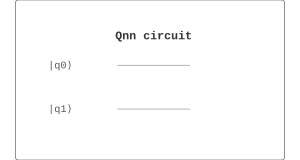
\includegraphics[width=0.6\textwidth]{../../images/qnn_circuit.svg}
\end{center}

\subsection{数学推导}

\textbf{Step 1: 量子态编码}

将经典数据 $x$ 编码为量子态：
\begin{equation}
|x\rangle = U_{\text{enc}}(x)|0\rangle^{\otimes n}
\end{equation}

其中 $U_{\text{enc}}$ 是编码电路。

\textbf{Step 2: 参数化量子电路}

应用参数化量子电路：
\begin{equation}
|\psi(\theta)\rangle = U_L(\theta_L) \cdots U_2(\theta_2) U_1(\theta_1)|x\rangle
\end{equation}

其中 $U_l(\theta_l)$ 是第 $l$ 层的参数化门。

\textbf{Step 3: 测量}

测量量子态得到输出：
\begin{equation}
f(x) = \langle\psi(\theta)|M|\psi(\theta)\rangle
\end{equation}

其中 $M$ 是测量算子。

\textbf{Step 4: 损失函数}

定义损失函数：
\begin{equation}
L(\theta) = \frac{1}{N} \sum_i (f(x_i) - y_i)^2
\end{equation}

\textbf{Step 5: 参数更新}

使用梯度下降更新参数：
\begin{equation}
\theta_{t+1} = \theta_t - \eta \nabla L(\theta_t)
\end{equation}

其中 $\eta$ 是学习率。

\subsection{几何解释}

量子神经网络在 Bloch 球上操作量子态。每一层参数化门旋转量子态，最终测量得到输出。

量子神经网络的参数空间是连续的，可以使用梯度下降优化。量子叠加允许网络同时探索多个参数路径。

\section{代码详解}

\begin{verbatim}
from quonic.ml import qnn

# qnn(data, labels, n_layers, learning_rate, epochs)
# data: 训练数据，形状为 (n_samples, n_features)
# labels: 标签，形状为 (n_samples,)
# n_layers: 量子电路层数
# learning_rate: 学习率
# epochs: 训练轮数

result = qnn(
    data=[[0, 1], [1, 0], [1, 1], [0, 0]],
    labels=[0, 1, 1, 0],
    n_layers=2,
    learning_rate=0.01,
    epochs=100
)

# result.accuracy: 准确率
# result.loss: 损失值
# result.params: 优化后的参数
# result.history: 训练历史
print(f'Accuracy: {result.accuracy}')
print(f'Loss: {result.loss}')
\end{verbatim}

\section{进阶用法}

\subsection{场景 1：不同层数}

\begin{verbatim}
from quonic.ml import qnn

# 不同层数的影响
for n in [1, 2, 3, 4]:
    result = qnn(data, labels, n_layers=n)
    print(f'n={n}: Accuracy={result.accuracy}')
\end{verbatim}

\subsection{场景 2：不同学习率}

\begin{verbatim}
from quonic.ml import qnn

# 不同学习率的影响
for lr in [0.001, 0.01, 0.1]:
    result = qnn(data, labels, learning_rate=lr)
    print(f'lr={lr}: Accuracy={result.accuracy}')
\end{verbatim}

\subsection{场景 3：多分类问题}

\begin{verbatim}
from quonic.ml import qnn

# 三分类问题
data = [[0, 1], [1, 0], [1, 1], [0, 0], [0.5, 0.5]]
labels = [0, 1, 2, 0, 1]

result = qnn(data, labels, n_layers=3)
print(f'Accuracy: {result.accuracy}')
\end{verbatim}

\section{适用场景}

\subsection{图像分类}

量子神经网络可以用于图像分类任务，如手写数字识别、人脸识别等。

\subsection{回归问题}

量子神经网络可以用于回归问题，如函数拟合、时间序列预测等。

\subsection{强化学习}

量子神经网络可以用于强化学习，如游戏 AI、机器人控制等。

\subsection{生成模型}

量子神经网络可以用于生成模型，如图像生成、数据增强等。

\section{常见问题}

\subsection{量子神经网络的表达能力如何？}

量子神经网络是通用逼近器，可以表示任意函数。对于 $n$ 个量子比特，可以表示 $2^n$ 维空间中的任意函数。

\subsection{量子神经网络需要多少量子比特？}

量子神经网络需要的量子比特数取决于特征维度。对于 $d$ 维特征，需要 $\lceil \log_2(d) \rceil$ 个量子比特。

\subsection{量子神经网络的训练时间如何？}

量子神经网络的训练时间包括：
\begin{itemize}
  \item 前向传播：$O(T_{\text{circuit}})$
  \item 梯度计算：$O(T_{\text{circuit}})$
  \item 参数更新：$O(1)$
\end{itemize}

其中 $T_{\text{circuit}}$ 是量子电路的执行时间。

\subsection{量子神经网络和经典神经网络有什么区别？}

量子神经网络使用量子门作为激活函数，可以在更高维的空间中表示函数。经典神经网络使用经典激活函数（如 ReLU、Sigmoid），受限于有限的函数类型。

\subsection{量子神经网络的收敛性如何？}

量子神经网络的收敛性取决于：
\begin{itemize}
  \item 学习率的选择
  \item 量子电路的深度
  \item 数据的质量
\end{itemize}

\section{学习路径}

\subsection{前置知识}
\begin{itemize}
  \item 神经网络基础
  \item 量子比特和量子门
  \item 量子测量
  \item 梯度下降
\end{itemize}

\subsection{继续学习}
\begin{itemize}
  \item 量子卷积神经网络（QCNN）
  \item 量子循环神经网络（QRNN）
  \item 量子生成对抗网络（QGAN）
  \item 量子强化学习（QRL）
\end{itemize}

\section{完整示例代码}

\subsection{示例 1：基本量子神经网络}

\begin{verbatim}
from quonic.ml import qnn

data = [[0, 1], [1, 0], [1, 1], [0, 0]]
labels = [0, 1, 1, 0]

result = qnn(data, labels, n_layers=2)
print(f'Accuracy: {result.accuracy}')
\end{verbatim}

\subsection{示例 2：带噪声的量子神经网络}

\begin{verbatim}
from quonic.ml import qnn

# 添加噪声
data_noisy = [[0 + 0.1, 1 - 0.1], [1 - 0.1, 0 + 0.1]]
labels_noisy = [0, 1]

result = qnn(data_noisy, labels_noisy, n_layers=2, noise=0.05)
print(f'Accuracy: {result.accuracy}')
\end{verbatim}

\section{下载}

\begin{itemize}
  \item [qnn.py](https://github.com/ChrisLee0721/QuoNic/blob/main/examples/qnn/qnn.py)
\end{itemize}

\end{document}
